\begin{figure*} 
	\begin{tabular}{c c c}
	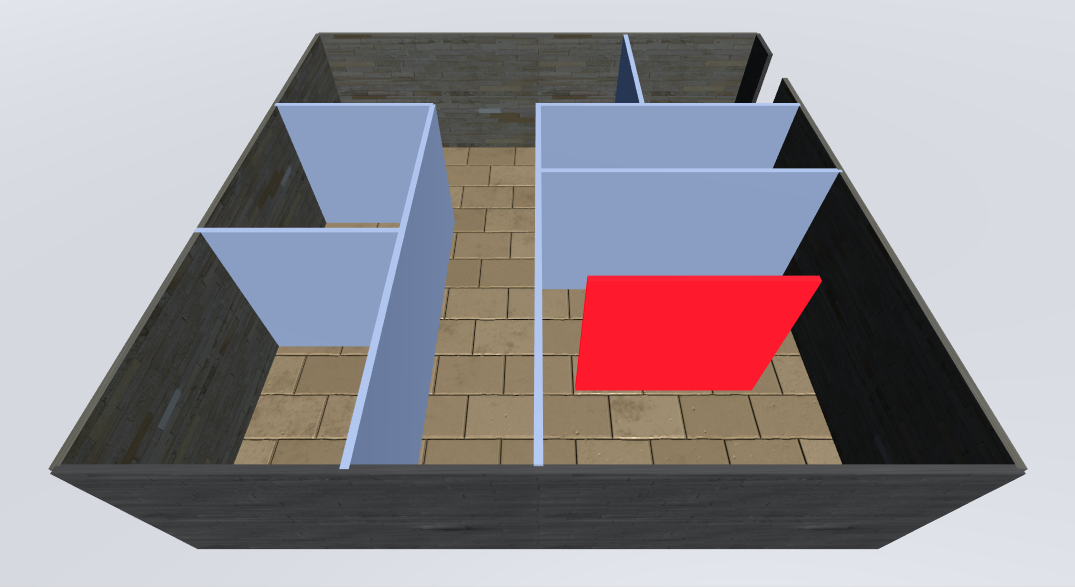
\includegraphics[width=0.31\textwidth]{images/InvalidWallPlacement.png} & 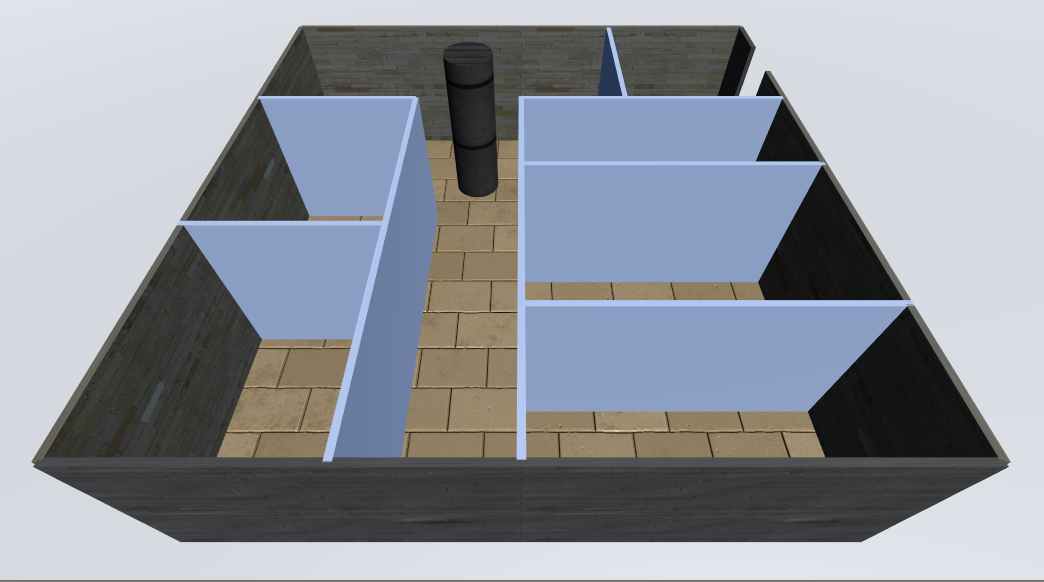
\includegraphics[width=0.31\textwidth]{images/ValidWallPlacement.png} & 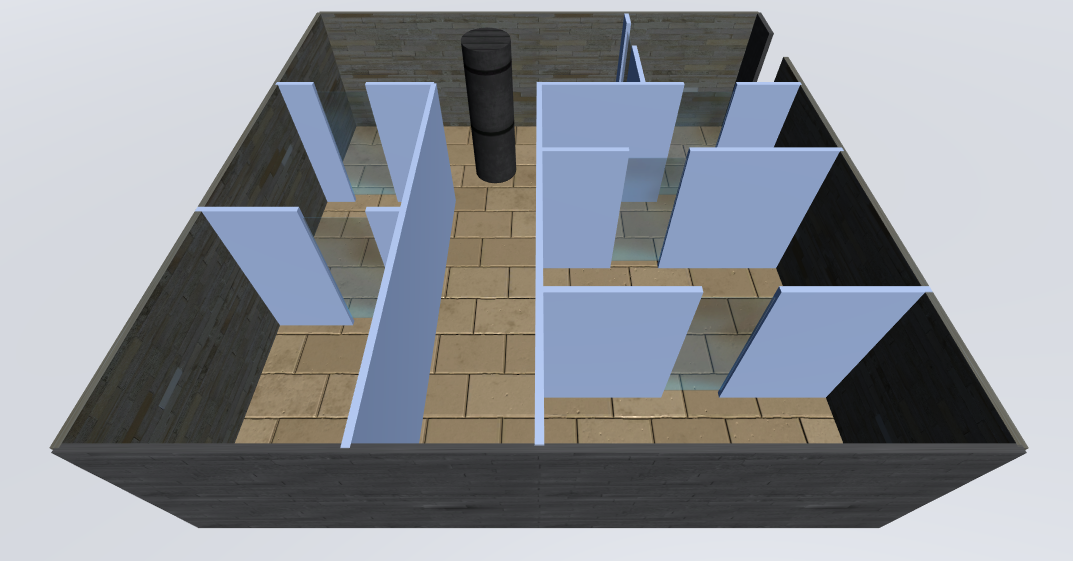
\includegraphics[width=0.31\textwidth]{images/ValidDoorAndPillarPlacement.png} \\
	(a) & (b) & (c)
	\end{tabular}
\caption{\label{fig:env-design}Environment design: a) invalid wall placement; b) wall placement c) door \& pillar placement.}  
\end{figure*}

The intention of gamifying architectural design is make the game usable by a player with any level of architectural knowledge. To meet these ends, the game framework provides a means of specifying and designing constraints/rules in the layout design phase of our game such that even casual player can achieve a layout which follows architectural standards.

Any architectural layout primarily comprises of walls, pillars, and doors. Hence we provide the tools to the the player to modify and create these elements in the layout. However, the game also provides the tools to create gamified levels with different forms of challenges. An architect or designer may choose to focus on an entire design, and formulate levels in terms constraints on available elements and modifications in increasing levels of difficulty.  The architect or designer may formulate levels in terms of seperate portions of a larger environment and sort them in increasing difficulty, e.g. from the bathroom area, to a common area, to a high traffic area, and so on. The architect or designer may also choose to iteratively incorporate more portions of the environment such that success criteria in the new level may be additive in terms of the previous design.  The gamification framework and level specification affords a number of options in order to lead player to producing designs for the architect or designer.  Display messages can be provided to help casual players learn about architectural standards when their design violate these constraints. Thus, the game can be used not just to produce design but also as an educational tool for novice designers or casual players.
